%\begin{wrapfigure}[0]{r}[-2.5cm]{3cm}
% \vspace{-6cm}
% \includegraphics[scale=0.4]{Schwingkreis/Bilder/schwingkreis.png}
% \vspace{-6cm}
%\end{wrapfigure}

\section*{Theorie- und Prüfungsfragen} 

\mucho{1}{TD203}
{Was ist im Resonanzfall bei der Reihenschaltung einer Induktivität mit einer Kapazität erfüllt?}%Frage
{Der Betrag des induktiven Widerstands ist dann gleich dem Betrag des kapazitiven Widerstands.}%A
{Der Wert des Verlustwiderstands der Spule ist dann gleich dem Wert des Verlustwiderstands des Kondensators.}%B
{Die Größe des elektrischen Feldes in der Spule ist dann gleich der Größe des elektrischen Feldes im Kondensators.}%C
{Die Größe des magnetischen Feldes in der Spule ist dann gleich der Größe des magnetischen Feldes im Kondensator.}%D
{A}%Lösung

\mucho{2}{TD209}
{Welche Resonanzfrequenz hat die Parallelschaltung einer Spule von 2 $\mu H$ mit einem Kondensator von 60 $pF$ und einem Widerstand von 10$k\Omega$?}%Frage
{145,288kHz}%A
{1,45288MHz}%B
{14,5288MHz}%C
{145,288 MHz}%D
{C \hspace{3em} $f_0 = \frac{1}{2 \pi \sqrt{L C}}$}%Lösung

\mucho{3}{TD206}
{ Wie ändert sich die Resonanzfrequenz eines Schwingkreises, wenn
1. die Spule mehr Windungen erhält, 2. die Länge der Spule durch Zusammenschieben der Drahtwicklung verringert wird, 3. ein Kupferkern in das Innere der Spule gebracht wird?}%Frage
{Die Resonanzfrequenz wird bei 1. und 2. kleiner und bei 3. größer.}%A
{Die Resonanzfrequenz wird in allen drei Fällen kleiner.}%B
{Die Resonanzfrequenz wird bei 1. kleiner und bei 2. und 3. größer.}%C
{Die Resonanzfrequenz wird bei 1. und 2. größer und bei 3. kleiner.}%D
{A}%Lösung


\mucho{4}{TD201}
{Der Impedanzfrequenzgang in der Abbildung zeigt die Kennlinie\\ 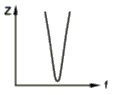
\includegraphics[scale=0.5]{Schwingkreis/Bilder/TD201.png}}%Frage
{eines Serienschwingkreises.}%A
{eines Parallelschwingkreises.}%B
{einer Induktivität.}%C
{einer Kapazität.}%D
{A}%Lösung

\vspace*{0.65cm}

\mucho{5}{TD202}
{Der Impedanzfrequenzgang in der Abbildung zeigt die Kennlinie\\
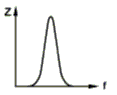
\includegraphics[scale=0.5]{Schwingkreis/Bilder/TD202.png}}%Frage
{eines Serienschwingkreises.}%A
{eines Parallelschwingkreises.}%B
{einer Induktivität.}%C
{einer Kapazität.}
{B}%Lösung

\aufgabentext{
	\begin{enumerate}
	\item[6] Um welche Schaltungen handelt es sich in folgender Abbildung.
	\end{enumerate}
	\loesung{1 Reihenschwingkreis, 2 Parallelschwingkreis, 3 Tiefpass, 4 Hochpass, 5 Bandpass, 6 Saugkreis, 7 Sperrkreis }
	}

\begin{figure}[H]
	\centering
	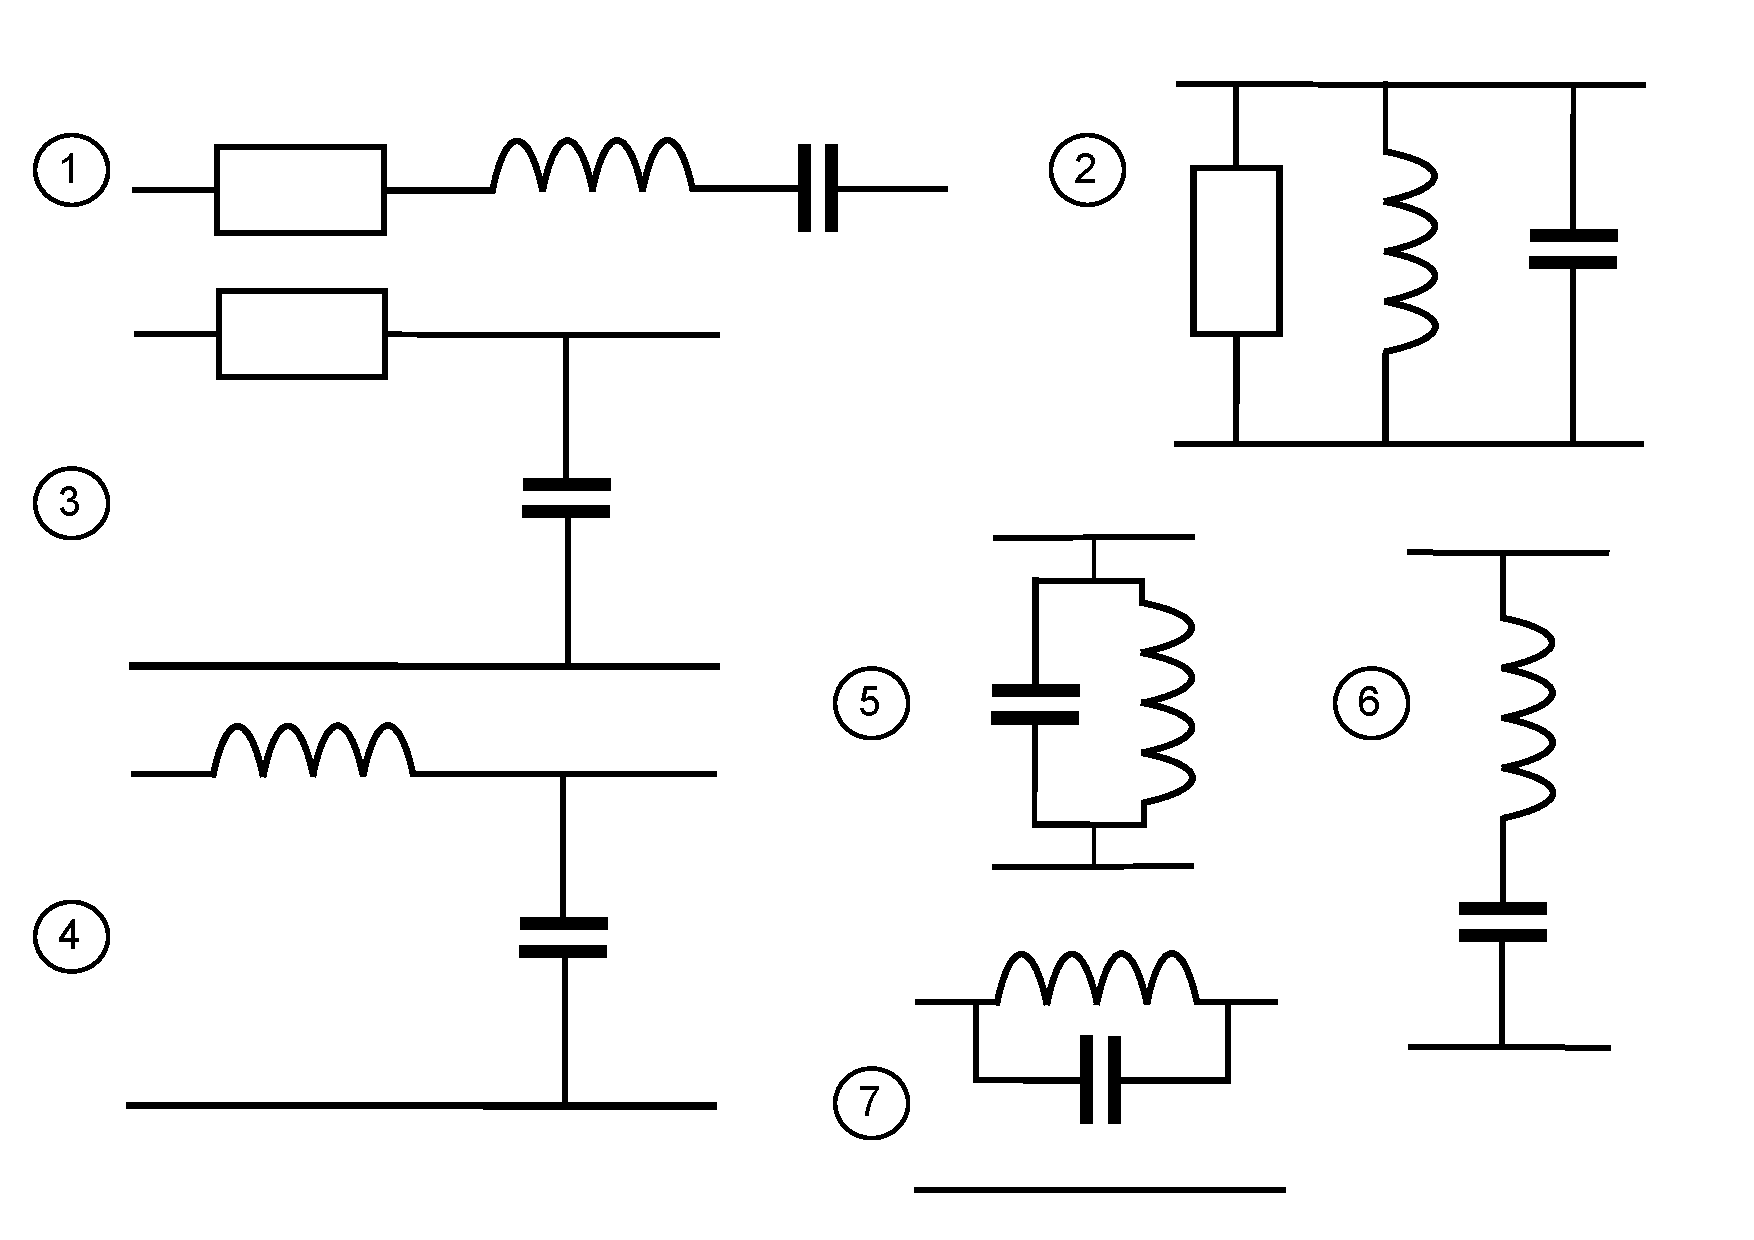
\includegraphics[scale=0.5]{Schwingkreis/Bilder/Filterschaltungen.pdf}
	\end{figure}

\mucho{7}{TD213}
{Welche Grenzfrequenz ergibt sich bei einem RC-Tiefpass mit einem Widerstand von 10$k\Omega$ und einem Kondensator von 50$nF$?}%Frage
{0,32$Hz$}%A
{318$Hz$}%B
{421$Hz$}%C
{318$kHz$}%D
{B \hspace{3em} $f_g = \frac{1}{2 \pi R C}$}%Lösung

\section*{Praxis}

\subsection*{Vorbereitung}

Seht euch die Pin-Belegung des Raspberry Pi (siehe Abbildung \ref{rpi}) sowie
die zu layoutende Schaltung für den 70cm-Tiefpassfilter (siehe Abbildung
\ref{70cmLP}) an. Wir benötigen GPIO18 und GND.

\begin{figure}[H]
    \centering
    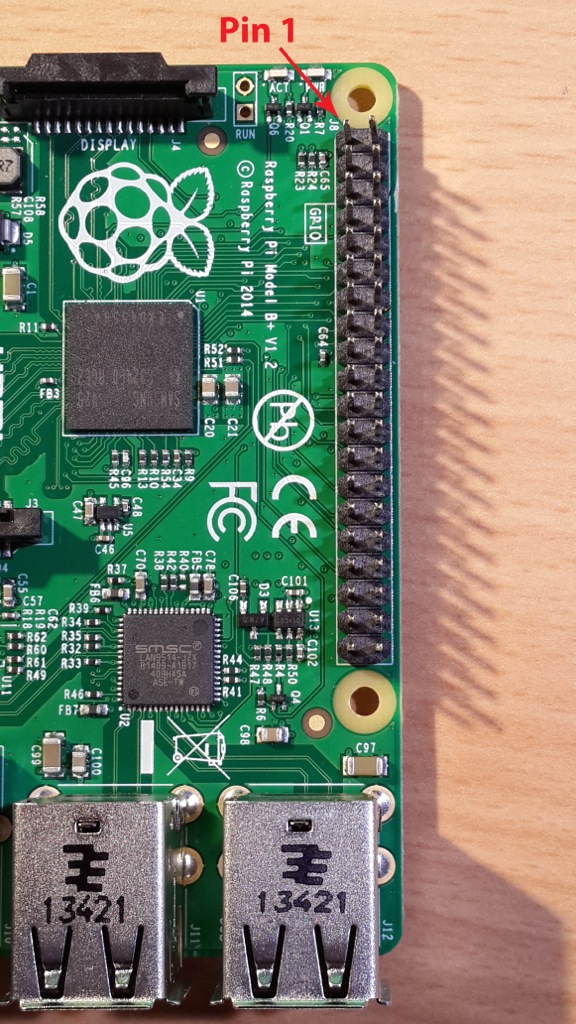
\includegraphics[height=0.4\textheight]{Schwingkreis/Bilder/B_plus_hdr_sm.jpg}
    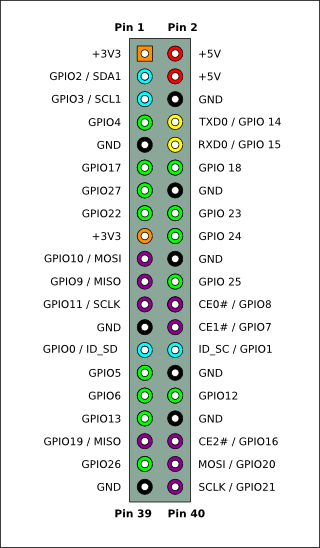
\includegraphics[height=0.4\textheight]{Schwingkreis/Bilder/Pi-GPIO-header.png}
    \caption{Connector pinout (P1 Header) -- Models B+, B2}
    \label{rpi}
    %FIXME Abbildungs-Quellenverzeichnis \url{http://elinux.org/RPi_Low-level_peripherals#Model_A.2B.2C_B.2B_and_B2}
\end{figure}

\begin{figure}[H]
    \centering
    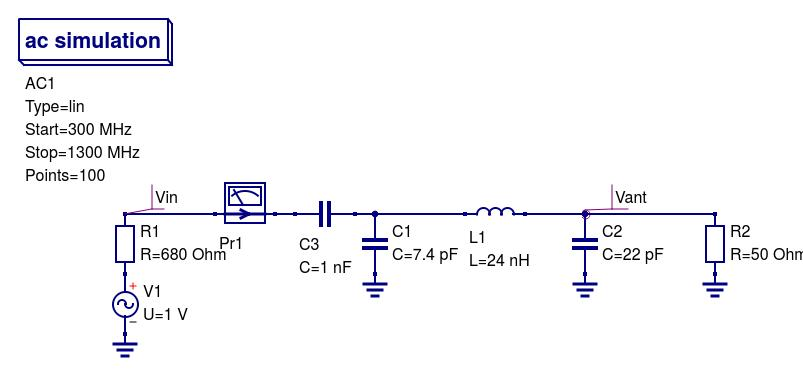
\includegraphics[width=1\textwidth]{Schwingkreis/Bilder/70cmLP500Ohm.jpg}
    \caption{Schaltung des 70cm-Tiefpassfilters aus Qucs}
    \label{70cmLP}
\end{figure}

\subsection*{Fritzing}

\subsubsection{Schematic View}

Bauteile aus den \emph{Core Parts} hinzufügen (fettgedruckte Bauteileigenschaften anpassen!):

\begin{itemize}
    \item  Basic
    \begin{itemize}
        \item Resistor $220 \Omega$ (THT)
        \item Inductor $22 nH$ (\textbf{SMD 1206})
        \item Ceramic Capacitor $1 nF$ (THT)
        \item Ceramic Capacitor $22 pF$ (THT)
    \end{itemize}
    \item  Input
    \begin{itemize}
        \item Variable Capacitor $2.1-10 pF$ (THT, \textbf{3.81mm pin spacing})
        \item Antenna (Wire soldering point)
    \end{itemize}
    \item Connection
    \begin{itemize}
        \item Generic female header (THT, \textbf{2x10}, \textbf{flip horizontal})
    \end{itemize}
    \item Schematic View
    \begin{itemize}
        \item Ground
    \end{itemize}
\end{itemize}

Nun können die Bauteile entsprechend des Schaltplanes "`verdrahtet"' werden.
\textbf{Hinweis}: Die Pin-Zählung des \emph{Generic female header} stimmt nicht
mit der des Raspberry Pi überein! Auf der Fritzing-Buchsenleiste gilt die
folgende Belegung:

\begin{itemize}
    \item GPIO = Pin 16
    \item GND = Pin 17
\end{itemize}

\subsubsection{PCB View}

\begin{itemize}
    \item PCB ändern auf \textbf{One Layer} \& Fäche ca. $30x30mm$
    \item Bauteile anordnen (THT-Bauteile auf Vorderseite, SMD auf Unterseite)
    \item Leitungen ziehen (es sollten nur die orangen Leitungen des unteren Layers zu sehen sein)
    \item Silkscreen Text mit dem Gruppennamen auf eine freie Fläche \\
          optional: Copper Fill Blocker \& Copper Text
    \item Rechtsklick auf einen Bauteile-Pin, der an Ground angeschlossen ist: "`Set Ground Fill Seed"'
    \item Menü $\rightarrow$ Routing $\rightarrow$ Ground Fill
\end{itemize}

\subsubsection{Zusatzaufgaben}

\begin{itemize}
    \item Antennenanschluss auf folgende MCX-Buchse umbauen: \\
          \url{http://www.reichelt.de/index.html?ARTICLE=152523}
    \item Testboard mit verschiedenen PCB-Spulen um ~24 nH erstellen, da typ. 2-3\% Abweichung. \\
          Berechnungsgrundlagen mit Online calculator:\\
          \url{http://coil32.net/pcb-coil.html}\\
          alternative Formen: \\
          \url{http://www.circuits.dk/calculator_planar_coil_inductor.htm}
\end{itemize}
